% !TEX root = ../gnss_interference_resistant_thesis.tex
\documentclass[main.tex]{subfiles}

\begin{document}

\subsection{Spindulio formavimo matavimai}\label{sec:beam_form_results}

\subsubsection{Spindulio formavimo matavimo stendas}

Spindulio formos matavimui naudojamas stendas pavaizduotas \ref{fig:beamform_stand}
pav. Pagrindiniai stendo elementai:

\begin{enumerate}
    \item HackRF siųstuvas, kuris generuoja CW signalą;
    \item 1x2 spinduolių sistema sudaryta iš GNSS signalams priimti skirtų antenų;
    \item Du HackRF koherentiniai imtuvai, susinchronizuoti anksčiau aptartais metodais;
    \item Siųstuvo stovas, kuris leidžia keisti siųstuvo kampą, spinduolių sistemos atžvilgiu;
\end{enumerate}

\begin{figure}[h]
    \begin{centering}
    \includegraphics[scale=1.0]{drawings/beamform_stand.drawio}
    \par\end{centering}
    \protect\caption{\label{fig:beamform_stand}Spindulio formos matavimo stendas.}
\end{figure}

Matavimai stendu pradedami vertikalioje padėtyje, įjungiamas siųstuvas ir abu imtuvai.
Atliekant signalų koreliaciją priimtų iš atskirų antenų, patikrinama laikinė sinchronizacija
ir randamas fazių skirtumas, kuris yra išsaugomas ir pritaikomas vienam iš imtuvų.

Spinduolių diagrama matuojama skaičiuojant priimamo signalo stiprumą: atliekama FFT
transformacija ir matuojamas maksimumo dydis. Nuskaičius vieną tašką, siųstuvo stovas
yra pasukamas iki kito kampo. Kampas yra matuojamas pasinaudoju išmaniojo telefono
akselerometro pagalba. Išmatavus vieno spinduolio diagramą įjungiamas spindulio formavimas
(signalų sudėtis) ir vėl kartojamas matavimas keičiant vieno iš imtuvo fazę.

% TODO add GNURADIO blocks

\subsubsection{Spindulio formavimo rezultatai}

Matavimai atliekami su 2 spinduolių sistema, pirmas matavimas atliekamas su viena
antena, antrasis - su dviem antenomis esant 0 fazės skirtumui ir trečias matavimas - su dviem
spinduoliais ir esant $2\ \mathrm{rad}$ fazės skirtumui. Spinduliai yra išdėstyti $\lambda / 2$ atstumu,
todėl esant $2\ \mathrm{rad}$ fazės skirtumui, tikimasi, kad diagramos maksimumas bus nukreiptas 40 laipsnių
kampu.

\begin{figure}[h]
    \begin{centering}
    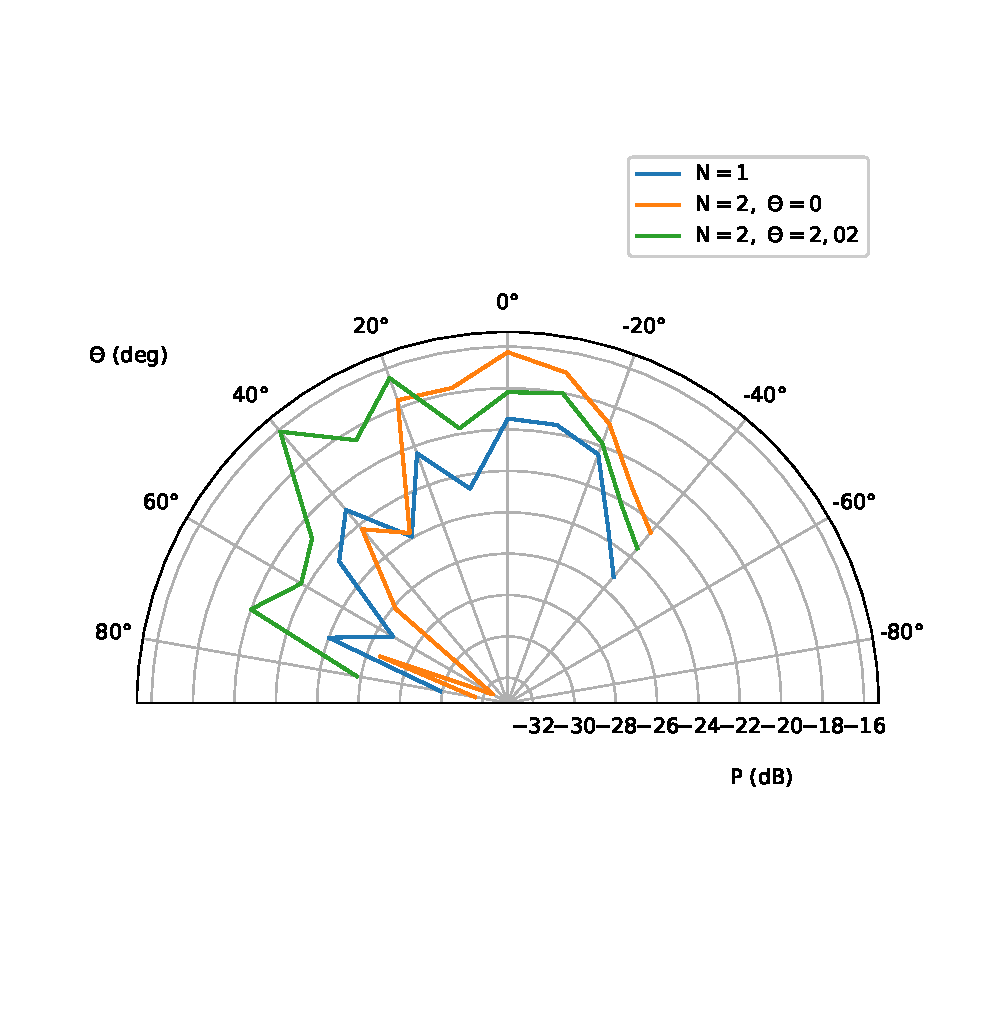
\includegraphics[scale=0.8]{drawings/beam_forming_results}
    \par\end{centering}
    \protect\caption{\label{fig:beamforming_result}Antenų sistemos spinduliavimo diagramos esant skirtingam spinduolių skaičiui
    ir skirtingai fazei tarp spinduolių.}
\end{figure}

Iš \ref{fig:beamforming_result}~pav. matome, kad naudojant viena spinduolį, diagramos maksimumas
yra $-19,4\ \mathrm{dB}$ ir yra nukreiptas 0 laipsnių kampu. Įjungus antrą anteną iškarto stebimas
$3\ \mathrm{dB}$ maksimumo padidėjimas iki $-16,4\ \mathrm{dB}$. Toks signalo padidėjimas reiškia,
kad priimama galia padidėjo 2 kartus, kadangi signalas priimamas iš dviejų antenų.

Vienam iš imtuvų pritaikius $\Delta \Theta = 2\ \mathrm{rad}$ fazės pokytį, gauta, kad
maksimumas pasislinko į 40 laipsnių kryptį, o signalo stiprumas išliko toks pat kaip atveju
kai fazės pokyčio
nebuvo. Šis rezultatas sutampa su \refeq{eq:phase_shift_antenna_angle} lygties rezultatu.

Visi matavimų grafikai turi tam tikrus minimumus, ten kur jų neturėtų būti. Jie atsiranda
dėl stovinčių bangų, kadangi matavimai buvo atlikti patalpoje nuo kurios sienų signalai
gali atsispindėti. Norint gauti tikslines spinduliavimo diagramas, matavimus reiktų
atlikti patalpoje, kurioje nėra atspindžių.

Iš gautų rezultatų galime daryti išvada, kad naudojant HackRF imtuvus spindulio formavimas
yra galimas, gaunamas $3\ \mathrm{dB}$ signalo sustiprėjimas ir pritaikius fazės pokytį,
galima keisti spinduolių sistemos kryptingumo diagramą.


\end{document}
